\documentclass[17pt]{extarticle}
\usepackage{amsmath, amssymb}
\usepackage{nccmath}
\usepackage[a4paper, total={8in, 11.38in},top=2mm,left=27mm,bottom=2mm,right=2mm]{geometry}

\usepackage{tikz}

\usepackage{titlesec}
\titleformat{\section}
{\normalfont\normalsize\bfseries}{\thesection}{1em}{}

\titleformat{\subsection}
{\normalfont\normalsize\bfseries}{\thesection}{1em}{}

\begin{document}

\noindent
\begin{fleqn} 

%%%%%%%%%%%%%%%%%%%%%%%%%%%%%%%%%%%%%%%%%%%%%%%%%%%%%%%%%%%%%%%%

\section{Question}
Show by vector method that the sum of the squares of the diagonals of a parallelogram is equal to the sum of the squares of its sides.
%----------------------------------------
\subsection*{Answer}
$\text{Let ABCD be a parallelogram with }$ \\
$\overline{AB} = \overline{DC} = \overline{a} \text{\;\;\;and}$\\
$\overline{BC} = \overline{AD} = \overline{b}$\\
%\vspace{-1.45cm}
\begin{equation} \nonumber
\begin{alignedat}{4}
\text{LHS } &= AC^2+BD^2 \\
&= |\overline{AC}|^2 + |\overline{BD}|^2\\
&= |\overline{AB}+\overline{BC}|^2 + |\overline{BC}+\overline{CD}|^2\\
&= |\overline{a}+\overline{b}|^2 + |\overline{a}-\overline{b}|^2\\
&= \\
&= \\
\end{alignedat}
%\vrule
%\vspace{1cm}
\quad\quad\quad
\begin{alignedat}{4}
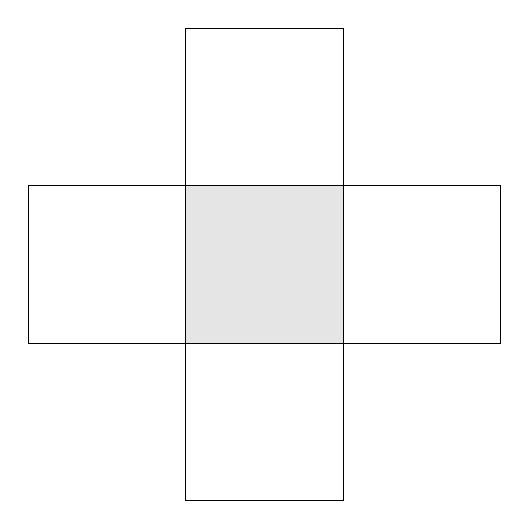
\begin{tikzpicture}
\draw (0,0) -- (0,2) -- (2,2) -- (2,4) -- (4,4) -- (4,2) -- (6,2) -- (6,0) -- (4,0) -- (4,-2) -- (2,-2) -- (2,0) -- (0,0) ; 
\filldraw[fill=gray!20] (2,0) rectangle (4,2);
\end{tikzpicture}
\end{alignedat}
\end{equation}
\quad
\vspace*{-5mm}

\begin{equation} \nonumber
\begin{alignedat}{4}
& \frac{dV}{dx}=\frac{1}{4}(300x - x^2) \\
& But\  \frac{dV}{dx}= 0 \text{ for max}\\
& \therefore \frac{1}{4}(300x - x^2)=0\\
& \therefore x = \pm 10\\
& \therefore x = 10 \ \ (+ve)
\end{alignedat}
\quad
\vrule
\quad
\begin{alignedat}{4}
&= \left(\frac{d^2V}{dx^2}\right)_{x=10}=\left(\frac{-3x}{2}\right)_{x=10} = -15<0\\
& \therefore \text{ V is max at x = 10 by 2nd derivative test}\\
& \therefore Height\  h=But\  \frac{300 - (10)^2}{4(10)}= 5\ cm\\
& \therefore Required\  dim = 5 \times  5 \times 10 \\
& Consequently \ Volume\ V = 500 \ cm^3 \\
\end{alignedat}
\end{equation}


%%%%%%%%%%%%%%%%%%%%%%%%%%%%%%%%%%%%%%%%%%%%%%%%%%%%%%%%%%%%%%%%

\section{Question}
The slant height of a right circular cone is 3 cm. Find the height of cone, if its volume is the greatest.

%----------------------------------------

\subsection*{Answer}
Let  r  and x  be the base-radius and the height of the cone respectively. Then the volume f(x) of the cone is given by

\begin{equation} \nonumber
\begin{alignedat}{4}
f(x) &= \frac{1}{3}\pi r^2x\\
&= \frac{\pi}{3}(3^2-x^2)x\\
&= \frac{\pi}{3}(9x - x^3)\\
\therefore f'(x) &=  \frac{\pi}{3}(9 - 3x^2)\\
\end{alignedat}
%\vrule
\quad\quad\quad
\begin{alignedat}{4}
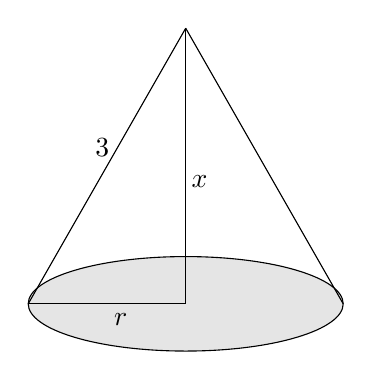
\begin{tikzpicture}
\filldraw[fill=gray!20](0,0) ellipse (2cm and 0.6cm);
\draw (0,0) -- node[below] {\ \ \ $x$}(0,3.5);
\draw (0,0)  -- node[below] {\ \ \ $r$} (-2,0);
\draw  (-2,0) --node[above] {3\ \ }(0,3.5);
\draw  (2,0) -- (0,3.5);
\end{tikzpicture}\\\\
\end{alignedat}
\end{equation}
\begin{equation} \nonumber
\begin{alignedat}{4}
& Now\ f'(x) = 0\ gives\\
& \frac{\pi}{3}(9x - x^3)=0\\
& \therefore \ 3x^2=9\\
& \therefore x = \sqrt{10}
\end{alignedat}
\quad
\vrule
\quad
\begin{alignedat}{4}
& Also\ \ f''(x) =-6x\\
& \therefore\ \ f''(\sqrt{3})=-6\sqrt{3}<0\\
& \therefore \ \ By\ second\ derivative\ test\\
& Volume \ f\ is maximum\ at\ x=\sqrt{3}
\end{alignedat}
\end{equation}
%%%%%%%%%%%%%%%%%%%%%%%%%%%%%%%%%%%%%%%%%%%%%%%%%%%%%%%%%%%%%%%%


\end{fleqn}
\end{document} 